\begin{frame}[c]{Définition}
\begin{block}{}
    \textbf{Protocole éditorial} = ensemble de règles \textit{explicites} et d'usages en vigueur au sein d'une structure éditoriale.\\
    \textrightarrow guider le processus de conception d'une publication.
\end{block}
\begin{block}{}
    Se présente souvent sous la forme d'une \textbf{série d'instructions précises et détaillées.}\\
\vspace{1em}
    L'ensemble des acteurs de la chaîne éditoriale sont soumis \textbf{au respect du protocole éditorial} (auteurs, éditeurs, préparateurs de copie, designer, directeurs artistiques, imprimeurs...).
\end{block}

\end{frame}

\begin{frame}{Un protocole négocié entre les acteurs et les outils de l'édition}
\begin{columns}[T,onlytextwidth]
\column{0.50\linewidth}
\small
\textrightarrow Détermine un \textbf{choix d'outillage} et donc des choix technologiques.\\
\vspace{1em}
\textrightarrow Vont aussi influencer, en retour, le protocole.
\column{0.50\linewidth}
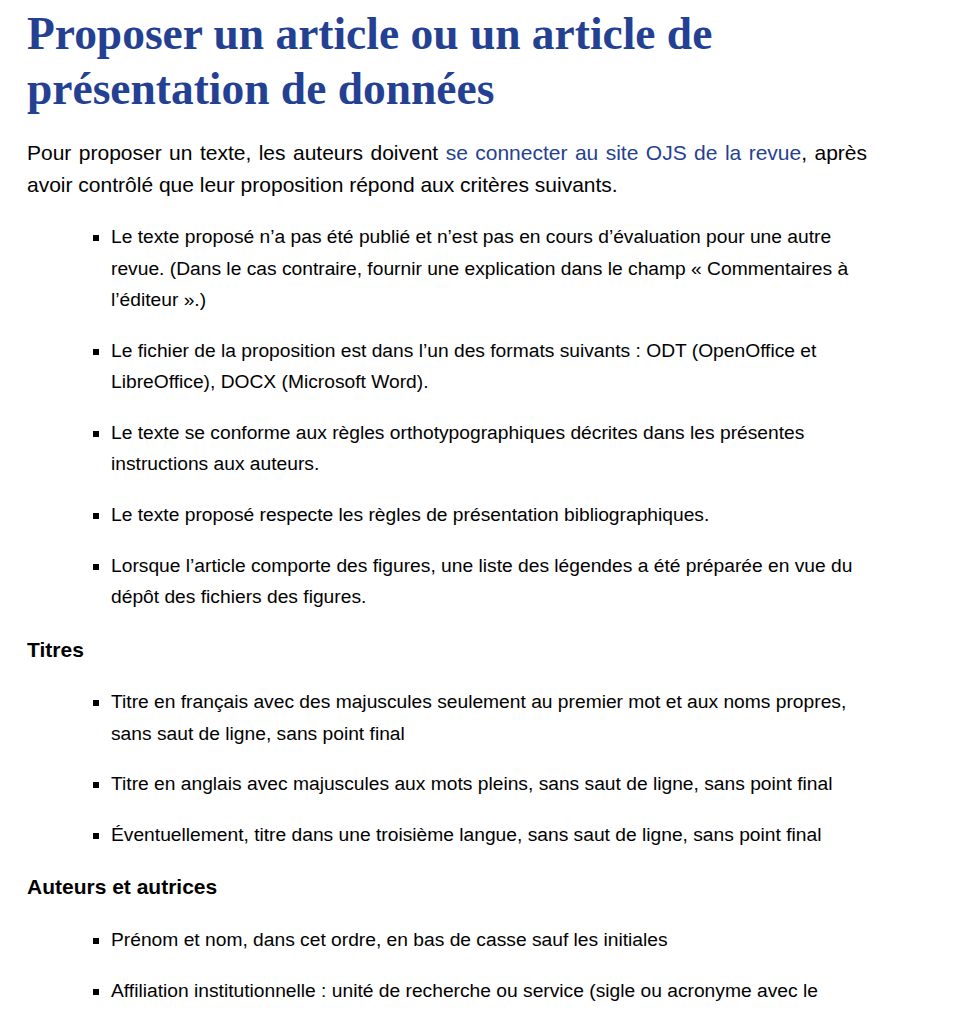
\includegraphics[width=.90\columnwidth]{05_Axe1_protocoles/images/protocole-hn-auteurs.png}
\end{columns}
    
\end{frame}